
\documentclass[a4paper, 10pt]{article}
\usepackage{a4wide}
\usepackage {amsmath}
\usepackage {graphicx}
\usepackage[utf8]{inputenc} 
\usepackage[francais]{babel}
\usepackage{fancyhdr}
\usepackage{setspace}
\usepackage{fancyhdr}
\usepackage{lastpage}
\usepackage{extramarks}
\usepackage{chngpage}
\usepackage{soul}
\usepackage[usenames,dvipsnames]{color}
\usepackage{graphicx,float,wrapfig}
\usepackage{ifthen}
\usepackage{listings}
\usepackage{courier}

\lhead{} 
\chead{} 
\rhead{\bfseries Intégration Numérique} 
\lfoot{JC Toussaint}
%\cfoot{} 
%\rfoot{\thepage}

% This is the color used for MATLAB comments below
\definecolor{MyDarkGreen}{rgb}{0.0,0.4,0.0}

% For faster processing, load Matlab syntax for listings
\lstloadlanguages{Matlab}%
\lstset{language=Matlab,                        % Use MATLAB
        frame=single,                           % Single frame around code
        basicstyle=\small\ttfamily,             % Use small true type font
        keywordstyle=[1]\color{Blue}\bf,        % MATLAB functions bold and blue
        keywordstyle=[2]\color{Purple},         % MATLAB function arguments purple
        keywordstyle=[3]\color{Blue}\underbar,  % User functions underlined and blue
        identifierstyle=,                       % Nothing special about identifiers
                                                % Comments small dark green courier
        commentstyle=\usefont{T1}{pcr}{m}{sl}\color{MyDarkGreen}\small,
        stringstyle=\color{Purple},             % Strings are purple
        showstringspaces=false,                 % Don't put marks in string spaces
        tabsize=5,                              % 5 spaces per tab
        %
        %%% Put standard MATLAB functions not included in the default
        %%% language here
        morekeywords={xlim,ylim,var,alpha,factorial,poissrnd,normpdf,normcdf},
        %
        %%% Put MATLAB function parameters here
        morekeywords=[2]{on, off, interp},
        %
        %%% Put user defined functions here
        morekeywords=[3]{FindESS, homework_example},
        %
        morecomment=[l][\color{Blue}]{...},     % Line continuation (...) like blue comment
        numbers=left,                           % Line numbers on left
        firstnumber=1,                          % Line numbers start with line 1
        numberstyle=\tiny\color{Blue},          % Line numbers are blue
        stepnumber=5                            % Line numbers go in steps of 5
        }

% Includes a MATLAB script.
% The first parameter is the label, which also is the name of the script
%   without the .m.
% The second parameter is the optional caption.
\newcommand{\matlabscript}[2]
  {\begin{itemize}\item[]\lstinputlisting[caption=#2,label=#1]{#1.m}\end{itemize}}

\pagestyle{fancy}

\begin{document}

\title{Application de l'intégration numérique en pluviométrie}

%\author{Jean-Christophe Toussaint\\
%  Phelma\\
 %\texttt{jean-christophe.toussaint@grenoble-inp.fr}
 %}
\date{\today}
 
\maketitle

Le but du B.E. est d'estimer la quantité totale de pluie tombée sur une région $D$ à partir
de mesures de pluviométrie faites sur un ensemble de noeuds distincts répartis sur $D$.

\section{Intégration d'une grandeur interpolée sur un domaine 1D}

Dans une première approche, on suppose que le domaine $D$ est unidimensionnel. 
On construit à partir des noeuds d'échantillonnage de la grandeur $Q(x)$, un 
maillage éléments finis à base de segments de droite (Fig. ~\ref{geo}).



\begin{figure}[ht]
\begin{center}$
\begin{array}{cc}
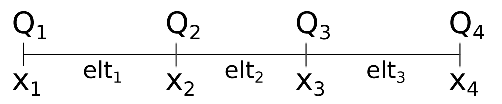
\includegraphics[scale=1, width=6cm]{sampling1D2.pdf} 
\end{array}$
\end{center}
\label{geo} 
\caption{décomposition du domaine en NE=3 éléments}
\end{figure}

%Soit $D$ un domaine de calcul unidimensionnel se limitant à un segment de droite. 
%On désire calculer l'intégrale $I=\int\limits_{D}\, Q(x)\, dx$ en décomposant le domaine
%de calcul $D$ en NE éléments finis de type P1(Fig. ~\ref{geo}).  

La description d'un maillage en éléments finis se fait, de manière générale, par 
l'intermédiaire de deux tableaux, la table des coordonnées et la table de connectivité.

La première contient les positions des noeuds. Ici, on lui adjoint
 les valeurs échantillonnées de $Q(x)$ aux noeuds:
\begin{table}[h] 
\centering 
\begin{tabular}{|c|c|c|}
  \hline
  noeud $i$ & abscisse $x_i$& $Q_i$ \\
  \hline
  1 & $x_1$ & $Q_1$ \\
  2 & $x_2$ & $Q_2$ \\
  3 & $x_3$ & $Q_3$ \\
  4 & $x_4$ & $Q_4$ \\
  \hline
\end{tabular}
\label{tab:hresult} 
\caption{table de coordonnées et des valeurs échantillonnées} %title of the table
\end{table}

La seconde table dite de connectivité associe à chaque élément $e$ la liste des NBN noeuds
lui appartenant:
\begin{table}[h] 
\centering 
\begin{tabular}{|c|c|c|}
  \hline
  élément $e$ &  I & II \\
  \hline
  1 & 1 & 2 \\
  2 & 2 & 3 \\
  3 & 3 & 4 \\
  \hline
\end{tabular}
\label{tab2:hresult} 
\caption{table de connectivité} %title of the table
\end{table}

La quantité de pluie intégrée, notée ci-après $I$, s'écrit comme une somme d'intégrales élémentaires sur chaque élément $e$:
\begin{equation}
I=\int\limits_{D}\, Q(x)\, dx=\sum_{e=1}^{NE} \int\limits_{e}\, Q_e(x)\, dx =\sum_{e=1}^{NE} I_e
\end{equation}

\begin{figure}[b!]
\begin{center}$
\begin{array}{cc}
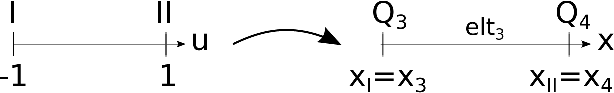
\includegraphics[scale=1, width=8cm]{elt_ref.pdf} 
\end{array}$
\end{center}
\label{eref} 
\caption{passage de l'élément de référence à l'élément réel}
\end{figure}

Pour calculer l'intégrale élémentaire $I_e$ sur un élément donné $e$, on lui associe
 un élément de référence (voir Fig. 2).

\begin{equation}
I_e=\int\limits_{e}\, Q_e(x)\, dx = \int\limits_{-1}^{1} Q(x(u))\, \frac{dx}{du}\,  du
\end{equation}

Pour simplifier, $Q(x(u))$ dans l'élément $e$, est noté dans la suite $Q_e(u)$.

Il faut ensuite définir la transformation géométrique $u \xrightarrow{T} x(u)$. La plus simple
est une transformation affine:

\begin{equation}
x(u)=x_I\, L_I(u) + x_{II}\, L_{II}(u)=\sum_{ie=I}^{NBN} x_{ie}\, L_{ie}(u)
\end{equation}

où $L_I=\frac{1-u}{2}$ et $L_{II}=\frac{1+u}{2}$.
Le déterminant jacobien associé à la transformation $T$ s'écrit : 
\begin{equation}
\frac{dx}{du} =\frac{x_{II}-x_{I}}{2}=detJ(u)
\end{equation}

On remarque que dans ce cas particulier d'éléments $1D$ affines par  morceaux ($P1$ de Lagrange), $detJ$ ne dépend pas de $u$. 

Pour effectuer l'intégration, on a besoin d'estimer $Q_e(u)$ en tout point de l'élément de référence. 
On l'approxime en effectuant une interpolation linéaire à partir de ses valeurs aux noeuds de l'élément.
Autrement dit:
\begin{equation}
Q_e(u)=Q_I\, L_I(u) + Q_{II}\, L_{II}(u)=\sum_{ie=I}^{NBN} Q_{ie}\, L_{ie}(u)
\end{equation}

L'estimation de l'intégrale élémentaire $I_e$ est calculée numériquement en utilisant la
méthode de Gauss:

\begin{equation}
I_e=\int\limits_{-1}^{1} Q_e(u)\, detJ(u)\,  du = \sum_{k=1}^{NPI} Q_e(u_k)\, w_k \, detJ(u_k)
\end{equation}

Après remplacement de $Q_e(u)$ par sa valeur interpolée, on obtient :

\begin{equation}
I_e= \sum_{k=1}^{NPI} \left( \sum_{ie=1}^{NBN} Q_{ie}\, L_{ie}(u_k) \right)\, w_k \, detJ(u_k)
\label{Ie_expr}
\end{equation}

Finalement, l'intégrale sur tout le domaine $D$ est obtenue après assemblage de toutes
les intégrales élémentaires $I_e$ :

\begin{equation}
I = \sum_{e=1}^{NE} I_e
\end{equation}

\textit{Remarque} : en 2D et 3D, on note $\alpha_{ie}(u)$ les polynômes de lagrange.

\section{Implémentation}
\subsection {Structure de données}

Le domaine d'intégration $1D$ est maillé avec des segments jointifs à $2$ noeuds. 
La structure $ \tt{fem }\rm$ contient la description complète du maillage. $ \tt{fem.NP }\rm$  et   $ \tt{fem.NE }\rm$ retournent respectivement le nombre total de noeuds et le nombre d'éléments. 

La table de coordonnées est implémentée sur la forme du tableau $ \tt{fem.noeud(1:fem.NP)} \rm$.
L'abscisse du noeud $\tt{np \in [1,   fem.NP \rm]}$ est donné par $ \tt{fem.noeud(np).x} \rm$. 

Le tableau $\tt{fem.elt(1:fem.NE)} \rm$ contient pour chaque élément $ \tt{ne}\rm$ :

\begin{itemize}
\renewcommand\labelitemi{\textbullet}
\item sa dimension $\tt{fem.elt(ne).TYP} \rm$,
\item  son nombre de noeuds $\tt{fem.elt(ne).NBN} \rm$,
\item le numéro de région $\tt{fem.elt(ne).NRG} \rm$ auquelle l'élément $ne$ appartient  et
\item  sa table de connectivité $\tt{fem.elt(ne).ind(ie)} \rm$ avec $\tt{ie \in [1,   fem.elt(ne).NBN \rm]}$
\end{itemize} 

Le tableau $\tt{fem.sol(1:fem.NP)} \rm$ contient l'échantillonnage de la grandeur à intégrer, en chaque noeud
du maillage.

Les données nécessaires pour le programme d'intégration, c'est à dire le maillage et les valeurs de la grandeur aux noeuds sont contenues dans le fichier $\tt{mesh.pro} \rm$. La lecture est effectuée par la fonction
$\tt{lecture\_probleme.m} \rm$

\matlabscript{lecture_probleme}{lecture des données du problème}

\matlabscript{mesh.pro}{fichier 'mesh.pro'}

\subsection {polynomes de Lagrange sur le segment à deux noeuds}

Pour chaque élément $\tt{ne} \rm$, la fonction $\tt{polynomes\_L2.m} \rm$ retourne une structure
de données $\tt{gauss} \rm$. Celle-ci contient comme données membres: le nombre de points d'intégration
(de Gauss) $\tt{NPI} \rm$ et pour chacun d'eux, la valeur du déterminant jacobien et le poids associé.

\matlabscript{polynomes_L2}{polynomes de Lagrange}

\section {Travail à réaliser}

\matlabscript{integrale}{integrale élémentaire}

Les taches à réaliser sont :

\begin{enumerate}
\item  Comprendre la structure du fichier $\tt{mesh.pro} \rm$ et les fonctions fournies.
\item Définir un algorithme de principe permettant de calculer de l'intégrale $I$ à partir
des intégrales élémentaires $I_e$.
\item Compléter la fonction $\tt{integrale.m} \rm$ qui effectue le calcul de l'intégrale élémentaire
selon l'équation \eqref{Ie_expr}.
\item Compléter la fonction  $\tt{solution.m} \rm$ qui somme les contributions de toutes les intégrales
élémentaires.
\item Exécuter le programme principal $\tt{PRECIPITATION\_main.m} \rm$ et modifier le fichier 
$\tt{mesh.pro} \rm$ pour valider le développement que vous avez réalisé.
\item  La fonction $\tt{polynomes\_L2.m} \rm$ utilise $2$ points de Gauss, est-ce bien nécessaire?
Justifier.
\end{enumerate} 

\matlabscript{PRECIPITATION_main}{programme principal}

\section {Extension}

On généralise l'étude pour calculer des intégrales de la forme $I_n=\int\limits_{D}\, Q(x)\, x^n\, dx$,
modifier le programme en conséquence. Comment se comporte-t-il en fonction de $n$? L'intégration de l'interpolée $P1$ de $Q(x)$ est-elle toujours exacte?
\end{document}

